\documentclass[12pt, a4paper, openany, twoside]{book}
\usepackage[italian]{babel}
\usepackage[T1]{fontenc}
\usepackage[utf8]{inputenc}
\usepackage{amsmath} 
\usepackage{xcolor}
\usepackage[margin=1in]{geometry}
\usepackage{hyperref}
\usepackage{pgfplots}
\usepackage{graphicx}
\graphicspath{{./img/}}
\hypersetup{
    colorlinks=true,
    linkcolor=blue,
    filecolor=magenta,      
    urlcolor=cyan,
}
%usepackage[latin1]{inputenc}
\begin{document}
\pagestyle{plain}
\author{DaveRhapsody}
\title{Prova di creazione grafici}
\date{3 Ottobre 2019}
\maketitle
\tableofcontents

%Prova inserimento immagine
Foto a cura di Letizia \\
$$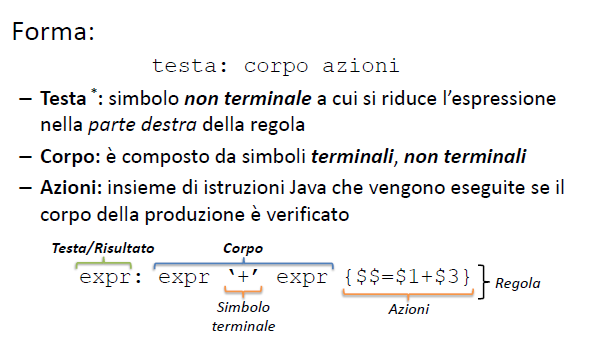
\includegraphics[width=0.50\textwidth]{2}$$
\end{document}